\documentclass{jsarticle}
\oddsidemargin=-0.8cm
\topmargin=-2cm
\baselineskip=13pt
\textheight=55\baselineskip
\marginparsep=0.5in
\marginparwidth=0.5in
\textwidth=52zw
\usepackage{ascmac}
\usepackage{url}
\usepackage[dvips]{graphicx}
\usepackage{amsmath}
\usepackage{amssymb}
\usepackage{multicol}
\usepackage{bm}
\usepackage{enumerate}
\usepackage{listings}
\usepackage{fancybox}
\usepackage{framed}
\usepackage{subfigure}
\usepackage{ccaption}
\usepackage{color}
\makeatletter
\lstset{% 
language={C}, 
frame=trbl,% 
basicstyle={\small},% 
identifierstyle={\small},% 
commentstyle={\small\ttfamily},% 
keywordstyle={\small\bfseries},% 
ndkeywordstyle={\small},% 
stringstyle={\small\ttfamily}, 
tabsize=2,
breaklines=true, 
frame=none,
columns=[l]{fullflexible},% 
numbers=left,% 
xrightmargin=0zw,% 
xleftmargin=3zw,% 
numberstyle={\scriptsize},% 
stepnumber=1, 
numbersep=1zw,% 
backgroundcolor={\color[gray]{.90}},
} 
\makeatother

\newenvironment{problems}
{
  \renewcommand\labelenumi{\doublebox{\arabic{enumi}}}
  \begin{enumerate}
}{
  \end{enumerate}
  \renewcommand\labelenumi{\arabic{enumi}.}
}

\pagestyle{empty}	

\begin{document}
\title{基礎気象学講義 復習問題} % ここは毎回同じ
\author{第2回} %authorの代わりに第何回かを入れる
\date{放射} %内容を記載する
\maketitle

\section{問題}

    \begin{problems}
    \item 次の文章を読んで、後の問いに答えなさい。
        \begin{screen}
        教科書P.14の図2.6におけるエネルギー配分の数値は現時点での代表的な見積もりの一例である。大気内や地表面における大気放射エネルギー配分は研究者により数\%の評価の差異がある。
        特に、雲や大気中の微粒子(一般に(A)と呼ばれる)が太陽放射量の吸収に及ぼす効果については不明な点が多い。\\
        一方で、このような放射エネルギー収支のバランスはあくまで全球について成り立つものであり、$_{(\mathrm{a})}$\underline{地域別あるいは季節別に見ると成り立たない}。
        下図に人工衛星により観測された大気上端における放射収支とアルベドの緯度分布を示す。
        \begin{center}
        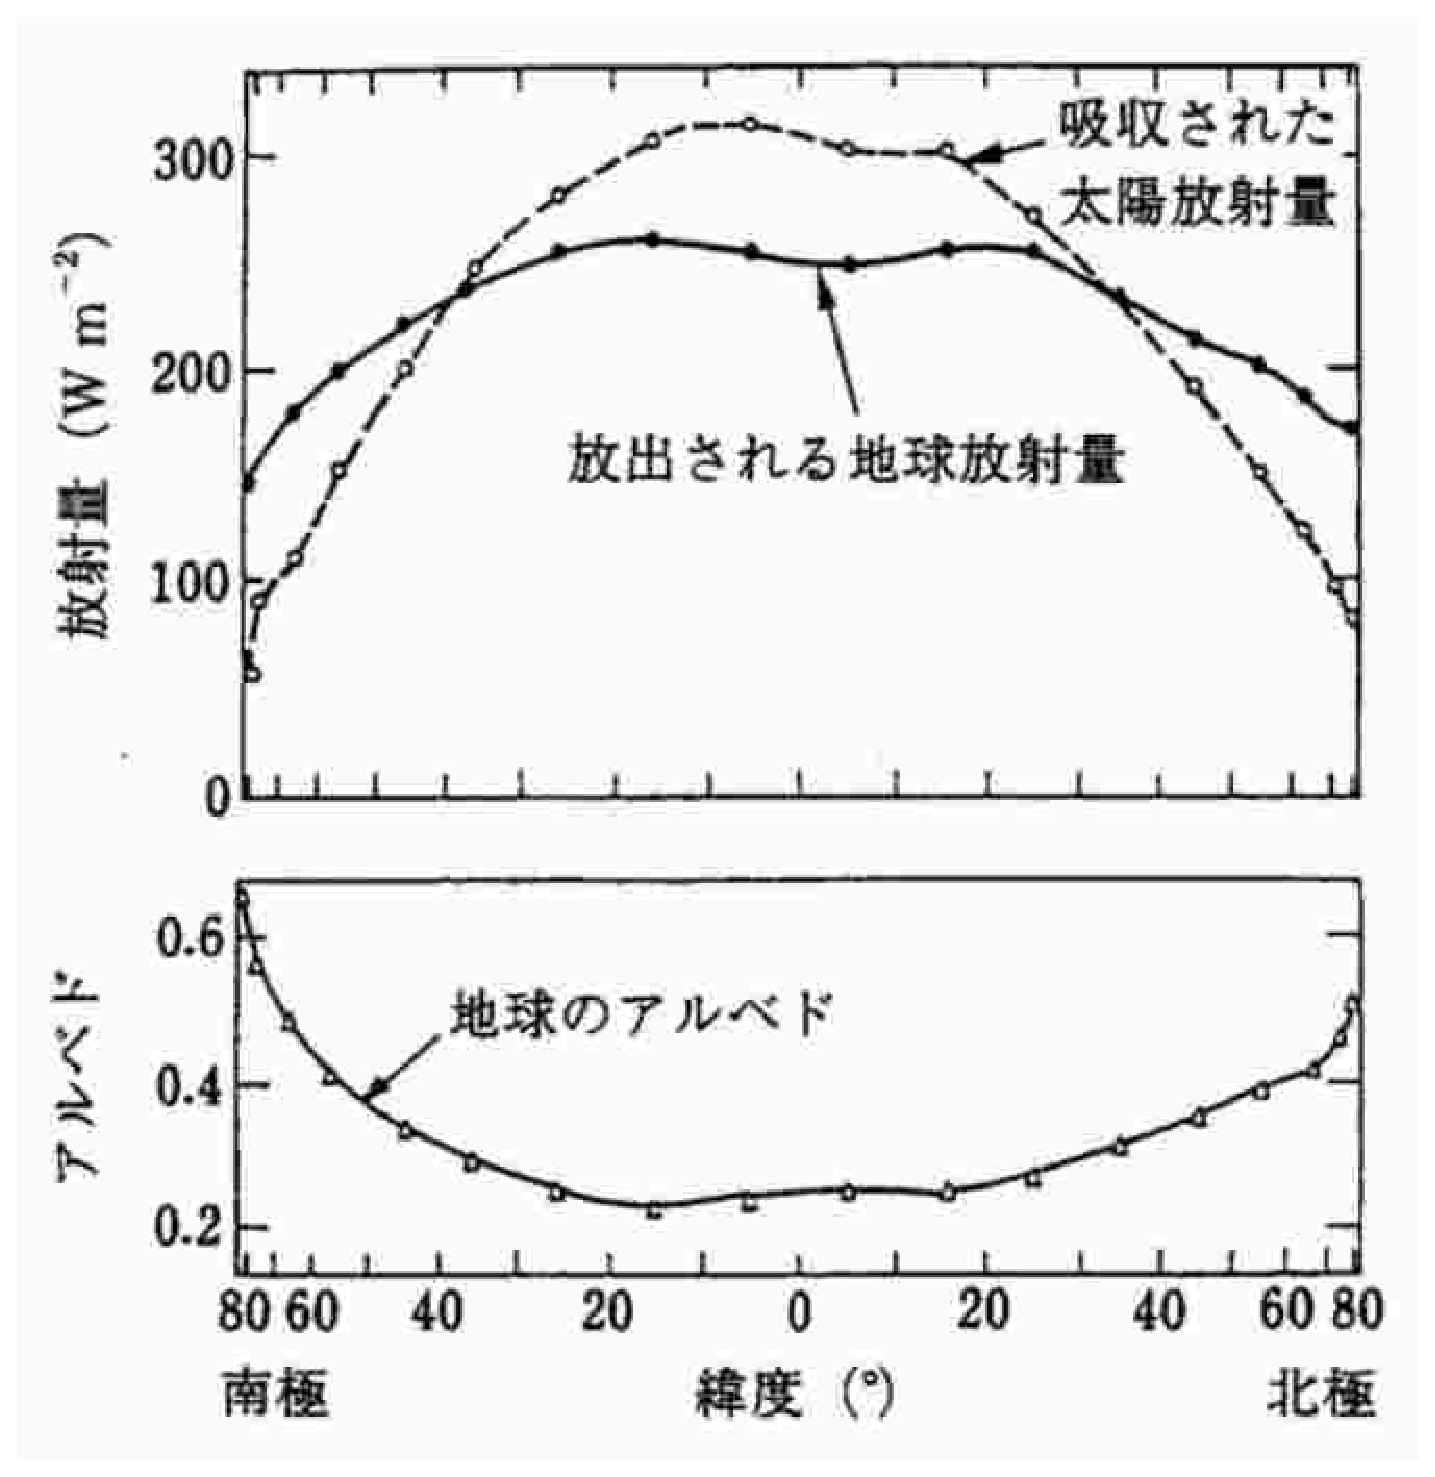
\includegraphics[width=0.5\linewidth,keepaspectratio]{AbsorbLat.eps}
        \end{center}

        図を見ると、南北とも概ね緯度(B)までは吸収量が多く、それより高緯度側では逆になる。この緯度方向の放射収支の不均衡は、放射過程がつねに低緯度側と高緯度側の温度差を拡大するように作用していることを示す。
        この温度差を縮小するように、大気や海洋の大規模な運動による(C)の輸送が起こる。\\
        このように放射エネルギーの収支は,大気と海洋の循環運動の平均状態としての気候の形成と深く結びついており、放射エネルギー分布のわずかの変調が気候の変化をもたらしうる。
        \begin{flushright}
            (講義テキストを元に作成・図は浅野「大気放射学の基礎」より引用)
        \end{flushright}
        \end{screen}

        \begin{enumerate}[(1)]
        \item 文中の空欄(A)〜(C)に当てはまる語句や数値を答えなさい。
        \item 下線部(a)のように、地域別あるいは季節別に収支バランスが成り立たない理由を述べなさい。
        \item アルベドの緯度分布は必ずしも南北対称とは言えない。対称でない理由を述べなさい。\\
        \end{enumerate}

    \item 地球に入射した太陽光は大気の粒子による吸収や散乱、また大気中あるいは地表の反射を経て地面に入射する。これについて、次の問いに答えなさい。
        \begin{enumerate}[(1)]
        \item 反射率は地表面の状態により変わるが、この反射率のことを何と言うか答えなさい。
        \item 雪面は古びて土が混ざるとよく溶けるとされるが、この理由を説明しなさい。
        \item 大気中での散乱には、大きくレイリー散乱とミー散乱がある。前者は波長より十分小さい球形粒子の電気双極子による2次放射、後者は波長と同程度の球形粒子による電磁波の散乱である。
              これらについて教科書を元に、性質を対比して一覧表にまとめなさい。
        \item 図\ref{Sahara}はサハラ砂漠上空で、人工衛星搭載の分光放射計で測定された地球放射のスペクトルを示している。
        \begin{figure}[h]
        \centering
        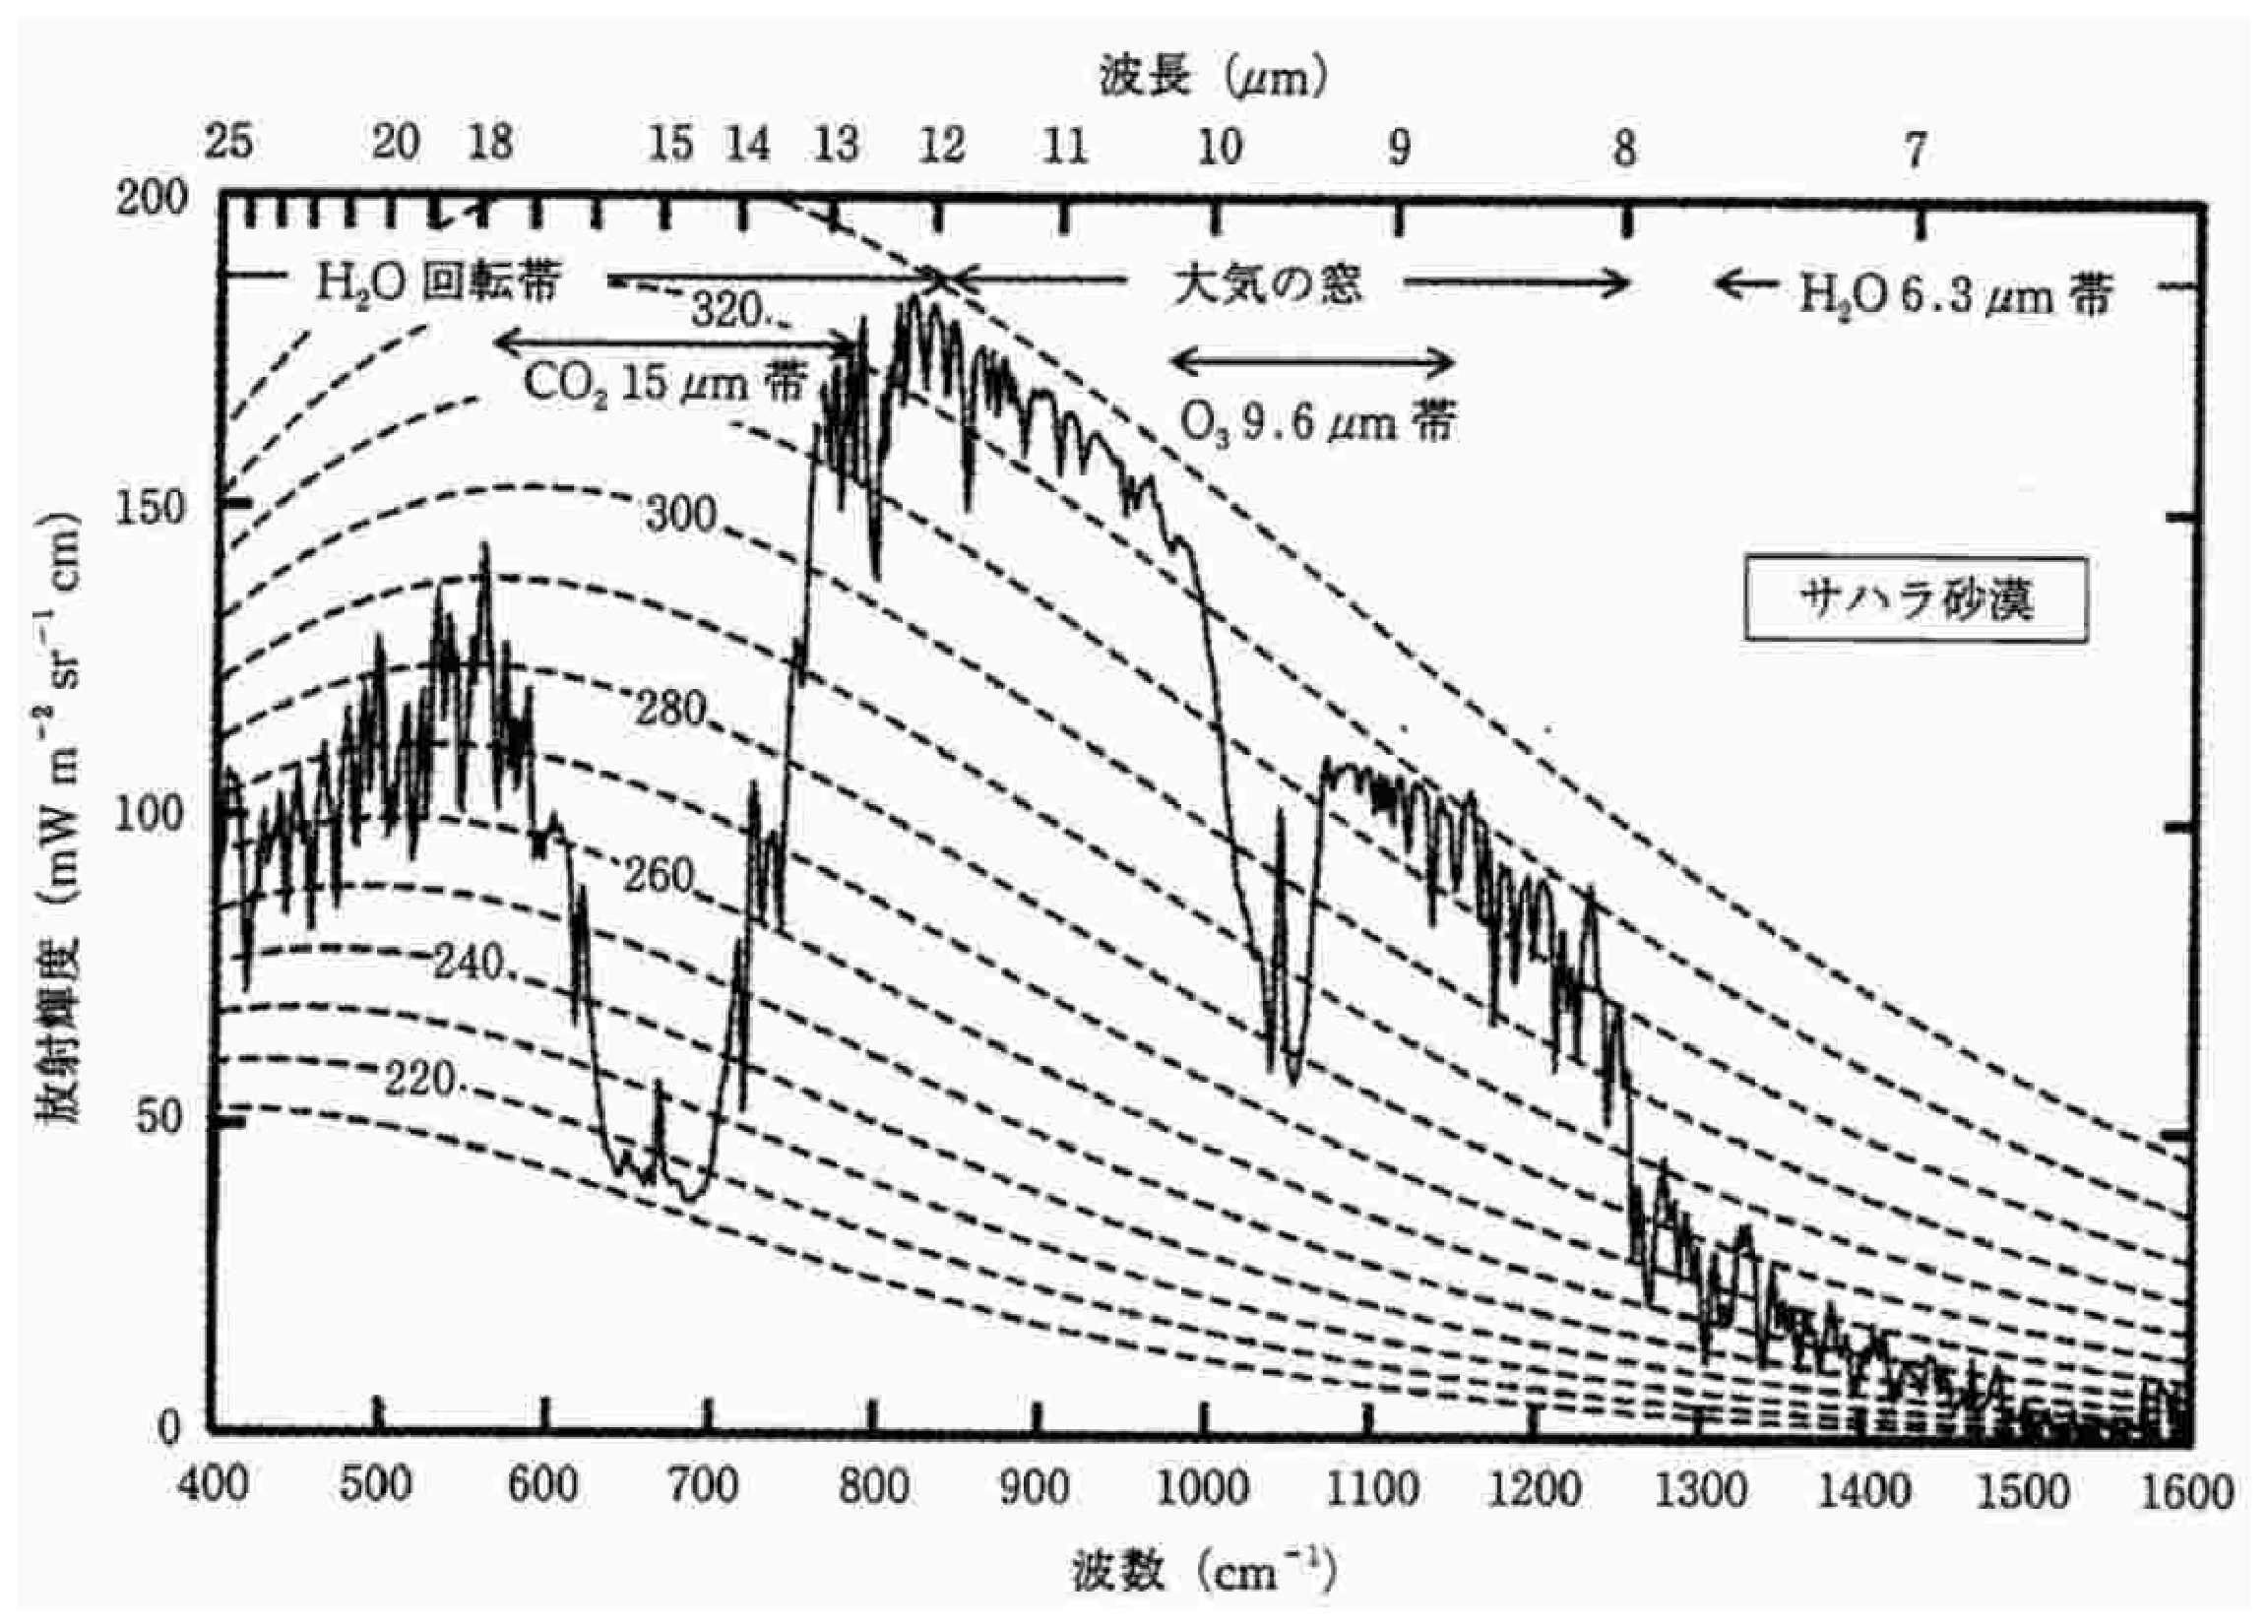
\includegraphics[width=0.6\linewidth,keepaspectratio]{Sahara.eps}
        \caption{地球放射スペクトル。破線は各温度での黒体放射スペクトル。(浅野「大気放射学の基礎」より引用)}\label{Sahara}
        \end{figure}
              地球放射に対して吸収量が勝るのはどの波長帯の部分か、図上部に書いてある○○帯(4つ)の中から全て選びなさい。
        \item 図\ref{Sahara}上部にある「大気の窓」領域とはどのような領域か説明しなさい。
        \item ある波長帯の赤外放射を吸収し、大気の昇温に寄与するような気体のことを何と言うか答え、その例を5例あげなさい。また、図\ref{Sahara}を元に、最もその寄与が大きい気体は何か答えなさい。
        \item 人間活動により、前問で答えた気体(寄与最大の気体を除く)が増加し、地表面温度が上昇する環境問題を何と言うか答えなさい。\\
        \end{enumerate}

    \item 黒体放射について、次の問いに答えなさい。
        \begin{enumerate}[(1)]
        \item 黒体とは何か、その定義を答えなさい。
        \item 黒体放射は等方的とされるが、等方的とはどういうことか説明しなさい。
        \item 黒体の放射輝度は、絶対温度$T$と波長$\lambda$の関数として、次式のプランク関数により与えられる。
        \begin{equation}
        B_{\lambda}(T)=\frac{2hc^2}{\lambda^5\{\exp(hc/k_B\lambda T)-1\}} \label{PlanckFunction}
        \end{equation}
        ここで、$c$は光速、$h$はプランク定数$6.62607\times 10^{-34}$Js、$k_B$はボルツマン定数$1.38065\times 10^{-23}$JK$^{-1}$である。
        これを全波長帯にわたって積分することで、シュテファン・ボルツマンの法則を導きなさい。また、シュテファン・ボルツマン定数を求めなさい。
        \item ある温度$T$においてプランク関数(\ref{PlanckFunction})の極大値を与える波長$\lambda _\mathrm{m}$を計算することにより、ウィーンの変位則を示しなさい。
        \end{enumerate}
\end{problems}

\section{答案}
\begin{problems}
% 以下に解答を作成してGit Push。
\item 
	\begin{enumerate}[(1)]
		\item
		\begin{enumerate}[(A)]
			\item エーロゾル
			\item 35
			\item 熱
		\end{enumerate}
		\item
		低緯度帯では、太陽からの正味の入射エネルギーは地球$\-$大気系から赤外放射として放出される量より多いが、高緯度帯だと逆になるから。
		\item
		地球の赤道面が軌道面と23.5度の角をもっているため、場所によって当たる量が違うから。
	\end{enumerate}

\item 
	\begin{enumerate}[(1)]
	\item
	アルベド
	\item
	古びて土が入るとアルベドが新しい雪に比べ、下がる。すなわち、熱が新しい雪よりも吸収しやすいため、溶けやすくなる。
	\item
\begin{table}[h]
\begin{tabular}{lll}
      & ミー散乱                    & レイリー散乱                      \\
散乱の違い & 入射放射の波長に比して粒子の半径が非常に小さい & 光の波長と粒子の半径が同じ程度の大きさであるときの散乱  \\
強さ    & 波長によらない                 & 波長の4乗に反比例                 \\
起こる場所 & 雲の近く                    & 大気                         
\end{tabular}
\end{table}
	\item
		$CO_2 15\mu m$帯、$H_2 O6.3\mu m$帯
	\item
		電磁波に対し、大気吸収の小さい波長帯・周波数帯のことを大気の窓という。
	\item
		温室効果ガス、\\	
			例)水蒸気、二酸化炭素($CO_2$)、メタン($CH_4$)、一酸化荷窒素($N_2O$)、六フッ化硫黄($SF_6$)\\
			最も寄与が大きい気体は水蒸気である。
	\item
		地球温暖化
	\end{enumerate}
\item 
	\begin{enumerate}[(1)]
	\item
		入射放射をすべて完全に吸収するという仮想的な物体を考えると、その物体の与えられた温度で理論上の最大エネルギーを放射する。このような仮想的物体を黒体という。
	\item
		黒体(ある対象)の性質、分布が方向に依存しないことである。
	\item

        	\begin{align*}
			      B_{\lambda}(T)=&\frac{2hc^2}{\lambda^5\{\exp(hc/k_B\lambda T)-1\}} \\
			      =& \int^\infty_0 \frac{2hc^2}{\lambda^5\{\exp(hc/k_B\lambda T)-1\}} d\lambda \\
            \frac{hc}{k_B\lambda T} = xより\\
            \frac{1}{\lambda} =& \frac{k_BT}{hc} x\\
            d\lambda =& -\frac{\lambda^2 k_BT}{hc} x\\
            =& 2ck_BT\int^\infty_0 \frac{1}{\lambda^3(e^x-1)}dx\\
            =& 2ck_BT\left(\frac{k_BT}{hc}\right)^3 \int^\infty_0 \frac{x^3}{e^x-1} dx\\
            ここで、\int^\infty_0 \frac{x^3}{e^x-1} dx = \frac{\pi^4}{15}となるので、\\
            =&\frac{2k_B^4T^4}{h^3c^2}\frac{\pi^4}{15}\\
            \frac{2k_B^4\pi^4}{15h^3c^2} = \sigma とおくと、\\
            =& \sigma T^4となる。\\
            また、\sigma =5.74 \times 10^{-12}となった。
        	\end{align*}
        \item
        \begin{align*}
                プランク関数(\ref{PlanckFunction})の微分が0となる条件を考える。積の微分法をすると、\\
          B'_{\lambda}(T) =& \frac{2hc^2}{exp^{hc/k_b\lambda T}} \left[-5 + \frac{exp^{hc/k_b\lambda T}hc}{\lambda k_BT(exp^{hc/k_b\lambda T})}  \right]\\
          となる。\\
          -5 + \frac{exp^{hc/k_b\lambda T}hc}{\lambda k_BT(exp^{hc/k_b\lambda T})} =& 0を考える。\\
          x = \frac{hc}{k_B\lambda T} とすると、\\
          \frac{x}{1-e^{-x}} =& 5となる。\\
          よって、\\
          \lambda =& \frac{hc}{xk_BT}となる。
        \end{align*}
  \end{enumerate}
\end{problems}

\section{読書案内}
学んだ分野についてより深める各論的な書籍を関係分野が一段落したときに紹介していく。
このコーナーで紹介する書籍は講義をより深める方向のものとし、講義レベル程度の参考書についてはシラバスを参照されたい。

大気放射に関する分野は邦書が充実しており、日本語で勉強しやすいと思われる。
\begin{itemize}
\item 浅野正二 2010 "大気放射学の基礎" 朝倉書店
\item グラント.W.ペティ 近藤豊,茂木信宏訳 2019 "詳解 大気放射学" 東大出版
\item Liou.K.N. 藤枝鋼,深堀正志 2014 "大気放射学" 共立出版
\item 会田勝 1982 "大気と放射過程" 東京堂出版
\end{itemize}

関連して、気象光学という分野もあり、邦書として以下を挙げておく。
\begin{itemize}
\item 柴田清孝 1999 "光の気象学" 朝倉書店
\end{itemize}

\end{document}

